\documentclass[11pt,a4paper]{article}

% ---------------------------------------------------------------------------
% MedSkel AI: the full guide, written to be read alone.
% Build:  latexmk -pdf medskel_guide.tex
% ---------------------------------------------------------------------------

\usepackage[T1]{fontenc}
\usepackage[utf8]{inputenc}
\usepackage{lmodern}
\usepackage[margin=2.3cm]{geometry}
\usepackage{amsmath,amssymb}
\usepackage{booktabs}
\usepackage{array}
\usepackage{xcolor}
\usepackage{tikz}
\usetikzlibrary{arrows.meta,positioning,shapes.geometric,calc}
\usepackage[most]{tcolorbox}
\usepackage{enumitem}
\usepackage{titlesec}
\usepackage{fancyhdr}
\usepackage[hidelinks]{hyperref}
\usepackage{parskip}

\definecolor{teal}{HTML}{0F8B8D}
\definecolor{ink}{HTML}{1E2A33}
\definecolor{soft}{HTML}{EEF6F6}
\definecolor{warn}{HTML}{B5532A}
\definecolor{warnbg}{HTML}{FBF0EA}
\definecolor{vessel}{HTML}{2BB673}

\color{ink}
\titleformat{\section}{\Large\bfseries\color{teal}}{\thesection}{0.6em}{}
\titleformat{\subsection}{\large\bfseries}{\thesubsection}{0.6em}{}
\setlist{itemsep=2pt,topsep=3pt}

\pagestyle{fancy}
\fancyhf{}
\fancyhead[L]{\small\color{teal}MedSkel AI --- the full guide}
\fancyhead[R]{\small\thepage}
\renewcommand{\headrulewidth}{0.3pt}

\newtcolorbox{remember}{colback=soft,colframe=teal,boxrule=0.6pt,arc=2pt,
  left=8pt,right=8pt,top=6pt,bottom=6pt,title={\bfseries Remember},fonttitle=\small,
  coltitle=white}
\newtcolorbox{honest}{colback=warnbg,colframe=warn,boxrule=0.6pt,arc=2pt,
  left=8pt,right=8pt,top=6pt,bottom=6pt,title={\bfseries Be honest about this},fonttitle=\small}
\newtcolorbox{example}[1][]{colback=white,colframe=teal!60,boxrule=0.5pt,arc=2pt,
  left=8pt,right=8pt,top=6pt,bottom=6pt,title={\bfseries Worked example#1},fonttitle=\small,
  coltitle=ink,colbacktitle=soft}
\newtcolorbox{prof}{colback=white,colframe=ink!40,boxrule=0.4pt,arc=2pt,
  left=8pt,right=8pt,top=5pt,bottom=5pt}

\newcommand{\grid}[1]{\begingroup\renewcommand{\arraystretch}{1.1}\begin{tabular}{|*{20}{c|}}\hline #1 \\\hline\end{tabular}\endgroup}

\begin{document}

% ---------------------------------------------------------------------------
\begin{titlepage}
\centering
\vspace*{3cm}
{\Huge\bfseries\color{teal} MedSkel AI\par}
\vspace{0.6cm}
{\Large Finding and measuring the blood vessels of the eye\par}
\vspace{0.4cm}
{\large The full guide, written to be read alone\par}
\vspace{2cm}
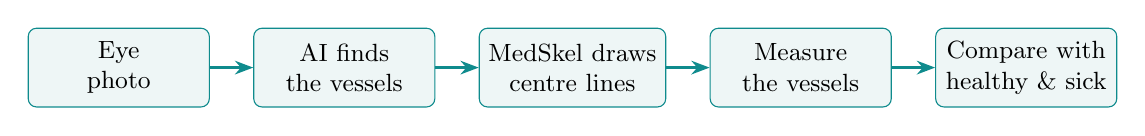
\begin{tikzpicture}[node distance=0.55cm, every node/.style={font=\small}]
  \tikzstyle{stp}=[rectangle,rounded corners=3pt,draw=teal,fill=soft,minimum width=2.3cm,minimum height=1.0cm,align=center]
  \node[stp] (a) {Eye\\photo};
  \node[stp,right=of a] (b) {AI finds\\the vessels};
  \node[stp,right=of b] (c) {MedSkel draws\\centre lines};
  \node[stp,right=of c] (d) {Measure\\the vessels};
  \node[stp,right=of d] (e) {Compare with\\healthy \& sick};
  \foreach \x/\y in {a/b,b/c,c/d,d/e} \draw[-{Stealth},thick,teal] (\x) -- (\y);
\end{tikzpicture}
\vfill
{\large Mouhssine El Boumshouli\par}
{EIDIA -- Université Euromed de Fès\par}
{Course: Réseaux de Neurones et Apprentissage Profond\par}
\vspace{0.3cm}
{\small November 2026\par}
\end{titlepage}

% ---------------------------------------------------------------------------
\section*{How to read this guide}
Read it in order. Each part builds on the one before. The parts are short.

\begin{itemize}
  \item Grey-green boxes called \textbf{Remember} hold the one idea you must keep.
  \item White boxes called \textbf{Worked example} show the maths with small numbers you can check by hand.
  \item Orange boxes called \textbf{Be honest about this} hold the limits. Say them in class. Professors trust students who know the limits of their own work.
  \item Part~11 has the questions your professor is likely to ask, with short answers.
  \item Part~12 is a small dictionary of the words used here.
\end{itemize}

Every number in this guide comes from your project's own results files (\texttt{report.md} and the \texttt{results/} folder on GitHub). Nothing is made up.

\tableofcontents
\newpage

% ---------------------------------------------------------------------------
\section{The big picture}

\subsection{The problem}
At the back of your eye there is a thin layer called the \textbf{retina}. It is full of tiny blood vessels. The eye is the only place in the body where a doctor can see blood vessels directly, without surgery: you just take a photo through the pupil. This photo is called a \textbf{fundus photograph}.

Some diseases change these vessels. Diabetes, high blood pressure and glaucoma are examples. So the vessels give doctors clues about a person's health. But looking at them by eye is slow, and two doctors can see the same photo differently.

\subsection{What the project does}
\begin{enumerate}
  \item \textbf{Find the vessels.} A neural network called a \textbf{U-Net} looks at the photo and marks every pixel that belongs to a vessel.
  \item \textbf{Draw the centre lines.} Your \textbf{MedSkel} method draws a thin line down the middle of every vessel, like a skeleton.
  \item \textbf{Measure.} From these lines we measure how much of the eye is covered by vessels, how long they are, how often they split, and how wide they are.
  \item \textbf{Compare.} We check whether these numbers look more like healthy eyes or sick eyes.
\end{enumerate}

\begin{remember}
\textbf{The one sentence:} the AI finds the vessels, MedSkel measures them, and the measurements are linked to eye disease. It is a research tool, not a diagnosis.
\end{remember}

\subsection{Where the project comes from}
You had an earlier project, \textbf{medskel}, that draws centre lines with geometry. Its weak point was the first step: it found the vessels with an old filter (the Frangi filter), which makes many mistakes. This new project replaces that filter with a CNN. A better drawing should give better measurements.

% ---------------------------------------------------------------------------
\section{How a computer sees a photo}

\subsection{A photo is a grid of numbers}
A photo is a grid of tiny squares called \textbf{pixels}. A FIVES photo is $2048 \times 2048$ pixels, so about 4.2 million pixels. Each pixel has three numbers between 0 and 255: how much \textbf{red}, \textbf{green} and \textbf{blue} it has. Black is $(0,0,0)$, white is $(255,255,255)$.

So for the computer, a photo is just a big table of numbers of size $2048 \times 2048 \times 3$.

\subsection{The answer is also a grid: the mask}
For every photo, an expert drew the vessels by hand. This drawing is called a \textbf{mask}. It has the same size as the photo, but each pixel holds only one number:
\[
1 = \text{this pixel is a vessel}, \qquad 0 = \text{it is not.}
\]
Here is a tiny $5\times5$ mask with one vessel going down and to the left:
\begin{center}
\grid{0&0&1&0&0\\\hline 0&0&1&0&0\\\hline 0&1&1&0&0\\\hline 0&1&0&0&0\\\hline 0&1&0&0&0}
\end{center}

\subsection{The task: segmentation}
The AI must look at the photo and produce its own mask, as close as possible to the expert's. Giving an answer \textbf{for every pixel} is called \textbf{segmentation}. This is harder than \textbf{classification}, which gives one answer for the whole image (for example ``this eye is sick'').

The network does not answer 0 or 1 directly. For each pixel it gives a \textbf{probability} between 0 and 1: how sure it is that the pixel is a vessel. Then we choose a \textbf{threshold}, for example 0.3: above it means vessel, below it means not a vessel.

\subsection{Why this is hard: few vessel pixels}
In FIVES, only about 7.5\% of the pixels are vessel. The rest is background.

\begin{example}[: the lazy model]
Imagine 100 pixels, of which 8 are vessel and 92 are not. A lazy model answers ``not a vessel'' for every pixel.
\begin{itemize}
  \item It is right on the 92 background pixels and wrong on the 8 vessel pixels.
  \item Its \textbf{accuracy} is $92/100 = 92\%$. That sounds great.
  \item But it found \textbf{zero} vessels. It is useless.
\end{itemize}
On the real FIVES test set, an all-black answer gets 92.9\% accuracy.
\end{example}

\begin{remember}
When one answer is much more common than the other, \textbf{accuracy lies}. That is why we judge the model with the \textbf{Dice score} (Part~6), which only looks at the vessels.
\end{remember}

% ---------------------------------------------------------------------------
\section{The data}

\subsection{FIVES: the main dataset}
FIVES is a public dataset published in 2022 in the journal \emph{Scientific Data}. It contains:
\begin{itemize}
  \item \textbf{800 eye photos}, each $2048\times2048$ pixels, all taken with the same kind of camera;
  \item \textbf{800 masks}, drawn by experts;
  \item four groups of 200 photos: \textbf{normal} (healthy), \textbf{AMD} (age-related macular degeneration), \textbf{diabetic retinopathy} (eye damage caused by diabetes) and \textbf{glaucoma}.
\end{itemize}
The authors already split it: 600 photos for training and 200 for testing.

\subsection{Three sets, like studying for an exam}
\begin{center}
\begin{tabular}{@{}lll@{}}
\toprule
\textbf{Set} & \textbf{Photos} & \textbf{Like\ldots} \\
\midrule
Training   & 510 & practice problems with the answers: the network learns from them \\
Validation & 88  & a practice exam: we use it to make decisions \\
Test       & 200 & the final exam: used only at the very end, for the honest score \\
\bottomrule
\end{tabular}
\end{center}

Why 510 and 88? From the 600 training photos, 2 masks were completely black (a mistake in the dataset), so we removed them. That leaves 598. We kept 88 of them aside for validation (22 from each group) and trained on the other 510.

\textbf{Why a validation set?} During the project we must make choices: when to stop training, which threshold to use, which improvement to keep. If we made these choices while looking at the test photos, the test would no longer be a surprise, and its score would look better than the truth. So every choice is made on the validation photos, and the test stays clean.

\subsection{CHASE\_DB1: the outside check}
CHASE\_DB1 is a small dataset from a different hospital and a different camera: 28 photos, both eyes of 14 children. Its special feature: \textbf{each photo was drawn by two different experts}. So we can measure how much two humans agree with each other, and compare the AI with that. We never trained on CHASE and never made any choice with it.

\begin{honest}
\begin{itemize}
  \item The 800 FIVES photos come from 573 patients, and the patients are not identified. The same person may have one eye in training and the other in the test. So our test score is a score on new \emph{photos}, not proven on new \emph{patients}.
  \item Six pairs of FIVES photos are exact copies of each other. We kept each pair on the same side of the split.
\end{itemize}
\end{honest}

\subsection{Photos are too big for the GPU: tiles}
Your laptop GPU (RTX 3050) has 4 GB of memory. A full $2048\times2048$ photo does not fit through the network at once. Shrinking the photo would make the thinnest vessels disappear. So we \textbf{cut it into tiles} of $512\times512$ pixels instead.
\begin{itemize}
  \item \textbf{Training:} the network sees random $512\times512$ pieces of full-size photos.
  \item \textbf{Prediction:} we cut the whole photo into overlapping tiles, predict each one, and stitch the results back together. Where tiles overlap, we average.
\end{itemize}

% ---------------------------------------------------------------------------
\section{The U-Net, piece by piece}

A \textbf{CNN} (convolutional neural network) is a neural network built from small filters that slide over an image. The \textbf{U-Net} is a famous CNN made for medical images in 2015. We will build it from its pieces.

\subsection{Piece 1: convolution (the filter)}
A filter is a small $3\times3$ grid of numbers. We put it on a $3\times3$ patch of the image, multiply each pair of numbers, and add everything up. That sum is one output number. Then we slide the filter to the next position and do it again.

\begin{example}[: a vertical line detector]
The filter, and two image patches:
\[
\text{filter} = \begin{pmatrix} -1 & 2 & -1\\ -1 & 2 & -1\\ -1 & 2 & -1 \end{pmatrix}
\qquad
\text{patch A} = \begin{pmatrix} 0 & 9 & 0\\ 0 & 9 & 0\\ 0 & 9 & 0 \end{pmatrix}
\qquad
\text{patch B} = \begin{pmatrix} 0 & 0 & 0\\ 9 & 9 & 9\\ 0 & 0 & 0 \end{pmatrix}
\]
\textbf{Patch A} (a vertical line): only the middle column is not zero, so the result is $3 \times (2\times9) = 54$. Strong answer.

\textbf{Patch B} (a horizontal line): the middle row gives $(-1)(9) + (2)(9) + (-1)(9) = 0$, and the other rows give 0. Result: $0$. No answer.

So this filter ``sees'' vertical lines and ignores horizontal ones.
\end{example}

The key points:
\begin{itemize}
  \item \textbf{We do not choose the filter numbers. The network learns them} during training (Part~5).
  \item The network uses many filters at once, for example 32. Each one produces its own output grid, called a \textbf{feature map}: one for edges, one for lines, one for dark spots, and so on. Vessels go in every direction, so the network learns filters for many directions.
  \item A colour photo has 3 layers (R, G, B), so a first-layer filter is really $3\times3\times3 = 27$ numbers, plus 1 extra number added at the end, called the \textbf{bias}: 28 learned numbers per filter.
  \item We add a border of zeros around the image (\textbf{padding}) so the output keeps the same size as the input.
\end{itemize}

\subsection{Piece 2: ReLU}
After each convolution, we keep positive numbers and turn negative numbers into zero:
\[
\text{ReLU}(x) = \max(0, x) \qquad\text{example: } [-3,\ 5,\ -1,\ 2] \;\to\; [0,\ 5,\ 0,\ 2].
\]
\textbf{Why?} A convolution only multiplies and adds. Ten convolutions in a row are, mathematically, the same as one big convolution, so stacking them would gain nothing. ReLU breaks this, and lets the network learn complicated shapes like curved, branching vessels.

\subsection{Piece 3: batch normalisation}
After each convolution, the numbers are rescaled so they stay in a similar range (around 0, with a similar spread). This makes training faster and more stable. You can think of it as keeping every layer's numbers ``at a comfortable size''.

\subsection{Piece 4: max pooling (shrinking)}
Cut the feature map into $2\times2$ blocks and keep only the biggest number of each block:
\[
\begin{pmatrix} 1 & 3 & 2 & 0\\ 4 & 2 & 1 & 1\\ 0 & 1 & 5 & 6\\ 2 & 0 & 7 & 3 \end{pmatrix}
\;\longrightarrow\;
\begin{pmatrix} 4 & 2\\ 2 & 7 \end{pmatrix}
\]
The map becomes 2 times smaller in each direction. \textbf{Why?}
\begin{itemize}
  \item The next filters now cover a bigger part of the original photo. To tell a real vessel from a random dark spot, you need to see what is around it.
  \item It is less work for the computer.
\end{itemize}
\textbf{The price:} we lose the exact position. We know there is a vessel ``around here'', but not on which exact pixel.

\subsection{Piece 5: upsampling (growing back)}
The opposite of pooling: the map is made 2 times bigger again (our U-Net uses \textbf{bilinear} upsampling, which fills the new pixels by smoothly blending their neighbours). The size comes back, but the fine detail lost in pooling does not come back by itself.

\subsection{Piece 6: skip connections (the key trick)}
On the way down, before each shrink, we \textbf{save} the feature maps. On the way up, when the map is back to the same size, we \textbf{stack} the saved maps next to the new ones. This is called \textbf{concatenation}.
\begin{itemize}
  \item The maps coming up from the bottom know \textbf{what} is there: ``a vessel is around here''.
  \item The saved maps from the way down know \textbf{where} exactly: ``the edge is on this pixel''.
  \item Together they give both. A few convolutions then mix them.
\end{itemize}
Without skip connections, the vessels come out blurry and too thick, and thin vessels disappear.

\subsection{Piece 7: the final answer for each pixel}
At the top, a last tiny $1\times1$ convolution turns the 32 feature maps into \textbf{one number per pixel}, called a \textbf{logit}. It can be any number, like $-3$ or $5$. The \textbf{sigmoid} function squeezes it into a probability between 0 and 1:
\[
\sigma(z) = \frac{1}{1 + e^{-z}} \qquad
\sigma(0) = 0.5,\quad \sigma(3) \approx 0.95,\quad \sigma(-3) \approx 0.05.
\]

\subsection{Putting it together: the U shape}
\begin{center}
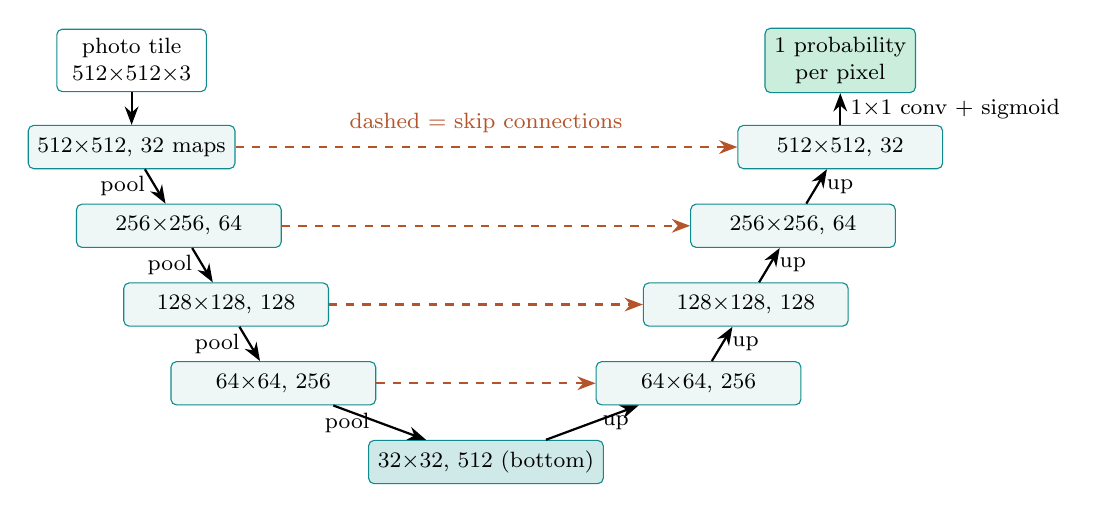
\begin{tikzpicture}[x=1cm,y=1cm,font=\footnotesize]
  \tikzstyle{blk}=[rectangle,draw=teal,fill=soft,minimum height=0.55cm,align=center,rounded corners=2pt]
  % encoder
  \node[blk,minimum width=2.6cm] (e1) at (0,0)    {512$\times$512, 32 maps};
  \node[blk,minimum width=2.6cm] (e2) at (0.6,-1) {256$\times$256, 64};
  \node[blk,minimum width=2.6cm] (e3) at (1.2,-2) {128$\times$128, 128};
  \node[blk,minimum width=2.6cm] (e4) at (1.8,-3) {64$\times$64, 256};
  \node[blk,minimum width=2.6cm,fill=teal!20] (b) at (4.5,-4) {32$\times$32, 512 (bottom)};
  % decoder
  \node[blk,minimum width=2.6cm] (d4) at (7.2,-3) {64$\times$64, 256};
  \node[blk,minimum width=2.6cm] (d3) at (7.8,-2) {128$\times$128, 128};
  \node[blk,minimum width=2.6cm] (d2) at (8.4,-1) {256$\times$256, 64};
  \node[blk,minimum width=2.6cm] (d1) at (9.0,0)  {512$\times$512, 32};
  \node[blk,minimum width=1.9cm,fill=vessel!25] (out) at (9.0,1.1) {1 probability\\per pixel};
  \node[blk,minimum width=1.9cm,fill=white] (in) at (0,1.1) {photo tile\\512$\times$512$\times$3};
  \draw[-{Stealth},thick] (in) -- (e1);
  \draw[-{Stealth},thick] (e1) -- node[left,pos=0.5]{pool} (e2);
  \draw[-{Stealth},thick] (e2) -- node[left]{pool} (e3);
  \draw[-{Stealth},thick] (e3) -- node[left]{pool} (e4);
  \draw[-{Stealth},thick] (e4) -- node[left]{pool} (b);
  \draw[-{Stealth},thick] (b) -- node[right]{up} (d4);
  \draw[-{Stealth},thick] (d4) -- node[right]{up} (d3);
  \draw[-{Stealth},thick] (d3) -- node[right]{up} (d2);
  \draw[-{Stealth},thick] (d2) -- node[right]{up} (d1);
  \draw[-{Stealth},thick] (d1) -- node[right]{1$\times$1 conv + sigmoid} (out);
  \foreach \a/\b in {e1/d1,e2/d2,e3/d3,e4/d4}
    \draw[-{Stealth},dashed,warn,thick] (\a.east) -- (\b.west);
  \node[warn,font=\footnotesize] at (4.5,0.3) {dashed = skip connections};
\end{tikzpicture}
\end{center}
The left side goes \textbf{down}: the image gets smaller but ``deeper'' (more feature maps). This side is the \textbf{encoder}. The right side goes \textbf{up} back to full size: the \textbf{decoder}. The skip connections are the bridges across the U. That is where the name comes from.

Each box on the way down is: convolution, batch norm, ReLU, convolution, batch norm, ReLU, then pooling. Our U-Net has \textbf{7,849,601 learned numbers} (called \textbf{parameters}) in total, and none of them were copied from another model: it was trained from scratch.

\begin{remember}
Encoder = understand \emph{what} is in the image (by shrinking). Decoder = rebuild the full-size answer. Skip connections = bring back \emph{where} things are, so the vessels stay sharp.
\end{remember}

% ---------------------------------------------------------------------------
\section{How the network learns}

At the start, all 7.8 million numbers are random, so the network's masks are nonsense. Training slowly changes the numbers until the masks look like the experts' masks.

\subsection{Step 1: measure how wrong it is (the loss)}
The \textbf{loss} is one number that says how wrong the network is. Lower is better. We use two losses and add them.

\textbf{Binary cross-entropy (BCE).} For each pixel, with $y$ the true answer (1 or 0) and $p$ the predicted probability:
\[
\text{BCE} = -\big[\, y \ln p + (1-y)\ln(1-p) \,\big]
\]
\begin{example}[: BCE on one vessel pixel ($y = 1$)]
\begin{itemize}
  \item The network says $p = 0.9$ (confident and right): $\text{BCE} = -\ln 0.9 \approx 0.11$. Small penalty.
  \item The network says $p = 0.1$ (confident and wrong): $\text{BCE} = -\ln 0.1 \approx 2.30$. Big penalty.
\end{itemize}
BCE punishes confident mistakes very hard.
\end{example}

\textbf{Dice loss.} BCE treats every pixel the same, and 92\% of pixels are background. So the network could get a low BCE by being lazy about vessels. The Dice loss fixes this: it only looks at how well the vessels overlap (Part~6), so it pays attention to the small vessel class.
\[
\text{Dice loss} = 1 - \text{Dice} \qquad \text{(0 = perfect overlap, 1 = no overlap)}
\]
Our loss is $\text{BCE} + \text{Dice loss}$, with equal weights. BCE gives stable learning pixel by pixel; Dice keeps the focus on the vessels.

\subsection{Step 2: find which way to change each number (backpropagation)}
Imagine you are on a hill in thick fog and want to reach the bottom. You cannot see the valley, but you can feel which way the ground slopes under your feet. So you take a small step downhill, feel again, take another step.

Training does the same. The ``height'' is the loss. \textbf{Backpropagation} is the method that computes, for each of the 7.8 million numbers, which direction makes the loss go down (this direction is called the \textbf{gradient}). It works backwards from the output to the input, layer by layer, using the chain rule from calculus.

\subsection{Step 3: take a step (Adam)}
Each number is changed a little in the downhill direction:
\[
w_{\text{new}} = w_{\text{old}} - \eta \times \text{gradient}
\]
$\eta$ is the \textbf{learning rate}, the size of the step. We started with $\eta = 0.001$ and lowered it smoothly to 0 by the end (small steps at the end, to settle in).

We use \textbf{Adam}, a smarter version of this rule. Adam remembers the direction of recent steps (like a ball that keeps rolling) and gives each number its own step size. It usually learns faster and more reliably.

\subsection{The training loop}
\begin{enumerate}
  \item Take a small group of tiles (a \textbf{batch}: here 4 tiles of $512\times512$, from 2 photos), randomly flipped, rotated or made a bit brighter or darker so the network sees more variety. This is called \textbf{data augmentation}.
  \item The network predicts their masks.
  \item Compute the loss against the experts' masks.
  \item Backpropagation computes the gradients.
  \item Adam updates all the numbers.
  \item Repeat thousands of times. One pass over the training data is called an \textbf{epoch}. After each epoch, we check the score on the validation photos and keep the best version.
\end{enumerate}

We also used \textbf{mixed precision}: some computations use shorter numbers, which saves memory and time on the GPU without hurting the result.

\subsection{What actually happened}
\begin{itemize}
  \item \textbf{Version 1:} 50 minutes of training on your RTX 3050, 38 epochs. Validation Dice went from about 0.53 at the start to 0.878 and then levelled off.
  \item \textbf{Version 2:} we tested improvements one at a time, always on the validation photos. Training 3 times longer (150 minutes) helped. Predicting each photo 4 times (normal, mirrored left-right, mirrored up-down, both) and averaging, called \textbf{flips}, also helped. A special loss for connected vessels (clDice loss) made things \emph{worse}, so we dropped it.
\end{itemize}

% ---------------------------------------------------------------------------
\section{How we know if it is good}

\subsection{Counting right and wrong pixels}
Compare the AI's mask with the expert's mask, pixel by pixel. There are four cases:
\begin{center}
\begin{tabular}{@{}lll@{}}
\toprule
 & \textbf{Expert says vessel} & \textbf{Expert says background} \\
\midrule
\textbf{AI says vessel} & TP (true positive): correct & FP (false positive): false alarm \\
\textbf{AI says background} & FN (false negative): missed & TN (true negative): correct \\
\bottomrule
\end{tabular}
\end{center}

\subsection{The scores}
\begin{align*}
\textbf{Dice} &= \frac{2\,TP}{2\,TP + FP + FN} &&\text{overlap of the two drawings (0 to 1)}\\[2pt]
\textbf{IoU} &= \frac{TP}{TP + FP + FN} &&\text{a stricter overlap score}\\[2pt]
\textbf{Precision} &= \frac{TP}{TP + FP} &&\text{of what the AI marked, how much is right}\\[2pt]
\textbf{Recall (sensitivity)} &= \frac{TP}{TP + FN} &&\text{of the real vessels, how many it found}\\[2pt]
\textbf{Specificity} &= \frac{TN}{TN + FP} &&\text{of the background, how much it left alone}
\end{align*}

\begin{example}[: Dice by hand]
The expert drew 12 vessel pixels. The AI marked 10 pixels, of which 8 are on the expert's vessels.
\[
TP = 8,\quad FP = 10 - 8 = 2,\quad FN = 12 - 8 = 4
\qquad\Rightarrow\qquad
\text{Dice} = \frac{2\times8}{2\times8 + 2 + 4} = \frac{16}{22} \approx 0.73
\]
The lazy model from Part~2 has $TP = 0$, so its Dice is 0, even with 92\% accuracy.
\end{example}

\textbf{Choosing the threshold.} The threshold (the probability above which a pixel counts as vessel) was chosen on the validation photos: 0.40 for version 1, and 0.30 for the final model with flips.

\textbf{Error bars.} A score on 200 photos is not exact. To know how much it could change with other photos, we use the \textbf{bootstrap}: we redraw the 200 photos at random (some twice, some not at all) 10,000 times, recompute the score each time, and keep the middle 95\%. That range is the \textbf{95\% interval}.

\subsection{The results}
\begin{center}
\begin{tabular}{@{}lll@{}}
\toprule
\textbf{Model} & \textbf{Test Dice (200 photos)} & \textbf{Note} \\
\midrule
Version 1 (50 min) & 0.875 & first model \\
Final U-Net (150 min + flips) & \textbf{0.889} (0.873 -- 0.903) & our main model \\
Pretrained U-Net (reference) & 0.907 (0.891 -- 0.921) & bigger, pretrained \\
\bottomrule
\end{tabular}
\end{center}

Final model on the FIVES test, by group: AMD 0.917, diabetic retinopathy 0.889, glaucoma 0.850 (the hardest), normal 0.902. Precision 0.919, recall 0.874.

\textbf{What the pretrained model is:} the same U-Net idea, but its encoder was first trained on 1.2 million everyday photos (ImageNet), so it starts with useful filters, and it is 3 times bigger. It beats our from-scratch model on FIVES. That is expected. Our model is the one you can explain fully.

\subsection{The outside check against two humans (CHASE\_DB1)}
\begin{center}
\begin{tabular}{@{}ll@{}}
\toprule
\textbf{Who is compared with expert 1} & \textbf{Dice} \\
\midrule
Our final model & 0.766 \\
Expert 2 (a human) & 0.777 \\
Pretrained model & 0.770 \\
\bottomrule
\end{tabular}
\end{center}
On photos from another camera, our model agrees with expert 1 almost as well as expert 2 does. But it makes a different kind of error: it marks \textbf{more} pixels as vessel than the experts (recall 0.908 vs 0.769 for the human, precision 0.66 vs 0.80). So it draws vessels too wide, or adds false ones.

\begin{honest}
\begin{itemize}
  \item The score drops a lot outside FIVES: from 0.889 to 0.766. The model works best on photos like the ones it learned from.
  \item It still misses many of the thinnest vessels: it finds only about \textbf{46\%} of the pixels of vessels 1 to 4 pixels wide.
  \item The FIVES test set was used twice (once for version 1, once for version 2), always after all choices were fixed.
  \item The three worst photos: one has an expert mask that does not match the photo (a mistake in the dataset), and two are very dark and blurry.
\end{itemize}
\end{honest}

% ---------------------------------------------------------------------------
\section{Your part: MedSkel centre lines}

\subsection{What a centre line is}
A vessel in the mask is a thick band of white pixels. To measure its length, or to count where it splits, we need a thin line running down its middle: the \textbf{centre line}, also called the \textbf{skeleton}.

\subsection{Two ways to draw it}
\textbf{Thinning (the standard method).} Peel pixels off the edges of the white band, layer by layer, until only a line 1 pixel wide is left. It is simple, but the result depends a lot on small bumps on the edges: a little bump becomes a little side branch.

\textbf{MedSkel (your method, from the 2024 paper by Saidou et al.).} Turn the outline of the vessel into a polygon (straight segments). The centre line is made of the points that are \textbf{at the same distance from both sides} of the vessel. This is computed with a geometric tool called a \textbf{Voronoi diagram}. Small bumps are smoothed away by the polygon, so the line is more stable.

\subsection{The measurements}
All lengths and widths are in \textbf{pixels}. We do not have a reliable way to convert them to millimetres.
\begin{center}
\begin{tabular}{@{}p{3.6cm}p{11cm}@{}}
\toprule
\textbf{Measurement} & \textbf{What it means} \\
\midrule
Vessel density & share of the retina covered by vessels (for example 11\%) \\
Fractal dimension & how richly the vessel tree branches and fills the space. A straight line has 1, a filled area has 2; eye vessel trees are around 1.5 \\
Total length & all centre lines added together \\
Branch points & how many times a vessel splits into two \\
Median width & the typical vessel width \\
Tortuosity & how twisty the vessels are (1 = straight). Not used for conclusions: it depends too much on the method \\
\bottomrule
\end{tabular}
\end{center}

\begin{honest}
While building this, we found a \textbf{bug in the original MedSkel code}: it measures vessel width only at a few points, mostly the vessel tips, where vessels are thin. A test vessel 12 pixels wide came out as 1.3 pixels. We did not change the original project. In the new project, width is measured the same way for both methods. Your old \emph{length} results are not affected by this bug.
\end{honest}

% ---------------------------------------------------------------------------
\section{What the measurements showed}

\subsection{How we compare two measurements}
We use the \textbf{relative difference}: $\dfrac{|a-b|}{\text{average of } a \text{ and } b}$.
\begin{example}[]
One drawing gives a total length of 100, another gives 120. Relative difference $= \frac{20}{110} \approx 0.18$, so 18\%.
\end{example}

\subsection{Check that the code is right}
On CHASE, between the two human experts, total length changes by 9.3\% with thinning and 3.2\% with MedSkel. These are \textbf{exactly the numbers your original project found}. So the new code is connected correctly.

\subsection{Result 1: MedSkel makes the AI's measurements more stable (FIVES)}
When the AI's drawing replaces the expert's drawing, how much do the measurements change?
\begin{center}
\begin{tabular}{@{}lcc@{}}
\toprule
\textbf{Measurement} & \textbf{Thinning} & \textbf{MedSkel} \\
\midrule
Total length & 6.8\% & 6.3\% \\
Branch points & 53\% & \textbf{26\%} \\
Width & 18\% & \textbf{13\%} \\
\bottomrule
\end{tabular}
\end{center}
With MedSkel, the number of branch points changes \textbf{half as much}. This is your method's strongest result.

\subsection{Result 2: an honest weakness (CHASE)}
On the other hospital's photos, the AI's measurements differ from the experts' \textbf{more} than the two experts differ from each other. For example, vessel density differs by 30\% (AI vs expert) against 13\% (expert vs expert). This comes from the over-marking seen in Part~6. The measurements do not yet transfer to a new camera.

\subsection{Result 3: sick eyes have different vessels (FIVES)}
Median values with the experts' drawings and thinning (about 200 photos per group):
\begin{center}
\begin{tabular}{@{}lcccc@{}}
\toprule
\textbf{Measurement} & \textbf{Healthy} & \textbf{AMD} & \textbf{Diabetic ret.} & \textbf{Glaucoma} \\
\midrule
Vessel density & 11.6\% & 10.0\% & 9.6\% & 9.4\% \\
Fractal dimension & 1.528 & 1.501 & 1.497 & 1.490 \\
Total length (px) & 30\,435 & 26\,620 & 23\,732 & 25\,159 \\
Branch points & 177 & 138 & 142 & 155 \\
\bottomrule
\end{tabular}
\end{center}
All three disease groups have less vessel area, a simpler tree, shorter vessels and fewer branch points than healthy eyes. The statistical tests say these differences are very unlikely to be luck ($p < 0.001$). A \textbf{p-value} is the chance of seeing a difference this big if there were really no difference; $p < 0.001$ means less than 1 in 1000.

\subsection{Can the measurements guess the group of one eye?}
We trained a simple model (logistic regression) on the measurements of the training photos, and tested it on the 200 test photos:
\begin{itemize}
  \item It guesses the right group (out of 4) about \textbf{45 to 49\%} of the time. Random guessing would get 25\%.
  \item Healthy vs diabetic retinopathy is easier: an AUC of about 0.84 with the AI's drawings (1.0 would be perfect separation, 0.5 is random).
\end{itemize}

\begin{remember}
The link between vessels and disease is \textbf{real for groups} (the averages clearly differ), but \textbf{too weak to diagnose one person} (wrong more than half the time). This is the same conclusion as large studies, like Yusufu et al.\ (2025) on about 10,000 people in the UK. Like height and age in children: older kids are taller on average, but you cannot tell a child's exact age from their height.
\end{remember}

\begin{honest}
These are links found in one dataset, not causes. Part of the difference may come from photo quality, from damage that hides vessels, or from how experts drew sick eyes. Nothing here can diagnose a patient.
\end{honest}

% ---------------------------------------------------------------------------
\section{The app}

\subsection{How to open it}
Double-click \texttt{MedSkel AI.bat} in the \texttt{medskel-ai} folder (or its desktop shortcut). A black window opens, then the app opens in your browser. Keep the black window open while you use the app; close it to stop the app.

\subsection{What you see}
\begin{enumerate}
  \item Upload an eye photo (or click one of the example photos) and press \textbf{Find and measure the vessels}.
  \item \textbf{The vessels:} a slider shows the photo on one side and the vessels in green on the other.
  \item \textbf{The centre lines:} the photo with MedSkel's centre lines in red.
  \item \textbf{The measurement table:} each value of this eye, the usual range for healthy eyes, and a sentence like ``lower than 82\% of healthy eyes''. Healthy eyes here means 50 healthy FIVES test eyes that went through exactly the same steps.
  \item \textbf{The chart ``Where does this eye sit?'':} for each measurement, the four groups as coloured bars and this eye as a red dot. You can see whether the eye looks more like healthy or sick eyes, and also how much the groups overlap.
  \item A button to download the numbers as a spreadsheet file (CSV).
\end{enumerate}

\textbf{Settings:} the threshold (default 0.30), the ``4 mirrored passes'' option (flips, slower but better), and ``resize to the training scale'' (keep it on, so pixels mean the same as in FIVES).

\subsection{How to present one eye in class}
``The AI found the vessels in a few seconds. MedSkel drew their centre lines. This eye has a vessel density of 9.9\%, lower than most healthy eyes, and on the chart the red dot sits inside the disease bars. But the bars overlap, so this is a clue for research, not a diagnosis.''

% ---------------------------------------------------------------------------
\section{The limits, in one place}
\begin{itemize}
  \item \textbf{Thin vessels:} only about 46\% of the thinnest vessel pixels are found.
  \item \textbf{Other cameras:} the score drops from 0.889 to 0.766 on CHASE, and the measurements do not transfer yet.
  \item \textbf{Pixels only:} no millimetres, so no real physical sizes.
  \item \textbf{One dataset:} the disease results come from FIVES only.
  \item \textbf{Patients:} we cannot prove that test patients were never seen in training.
  \item \textbf{One training run:} with one random seed.
  \item \textbf{Not a medical device:} it cannot diagnose anyone.
\end{itemize}

\textbf{What could come next:} more training to fix the over-marking on new cameras, better thin-vessel detection, a pixel-to-millimetre scale, and, one day, a study with a hospital using real patient records.

% ---------------------------------------------------------------------------
\section{Questions your professor may ask}

\begin{prof}\textbf{Q: Why not just use accuracy?}\\
Because 92\% of pixels are background. A model that marks nothing gets 92.9\% accuracy on FIVES and finds no vessel. Dice only looks at the vessels.\end{prof}

\begin{prof}\textbf{Q: What does a convolution do?}\\
It slides a small grid of learned numbers over the image, multiplies and adds. Each filter reacts to one pattern, like a vertical line. The network learns the filter numbers during training.\end{prof}

\begin{prof}\textbf{Q: Why does a U-Net need skip connections?}\\
Pooling loses exact positions. Skip connections bring back the detailed maps from the way down, so the decoder knows both \emph{what} is there and \emph{where}. Without them the vessels would be blurry and thin ones would disappear.\end{prof}

\begin{prof}\textbf{Q: Why BCE plus Dice loss?}\\
BCE gives stable learning for every pixel but is dominated by the background. Dice loss focuses on the overlap of the vessels, the small class. Together they work better than either alone.\end{prof}

\begin{prof}\textbf{Q: What is backpropagation?}\\
The method that computes, for every weight, which way to change it to lower the loss, working backwards through the layers with the chain rule. Then Adam takes a small step in that direction.\end{prof}

\begin{prof}\textbf{Q: Why a validation set if you have a test set?}\\
All choices (threshold, when to stop, which improvement to keep) are made on validation. The test set is used only at the end, so its score stays honest.\end{prof}

\begin{prof}\textbf{Q: How do you handle 2048-pixel images on a 4 GB GPU?}\\
We train on random $512\times512$ tiles of full-size photos and predict whole photos tile by tile with overlap, then stitch. Shrinking would erase thin vessels.\end{prof}

\begin{prof}\textbf{Q: Why is the pretrained model better, and why keep yours?}\\
It starts from filters learned on 1.2 million photos and is 3 times bigger, so it reaches 0.907 vs 0.889. Ours is trained from scratch and fully explainable. On CHASE both are equal (0.770 vs 0.766), so size was not the real limit there.\end{prof}

\begin{prof}\textbf{Q: Is your model as good as a human?}\\
On CHASE it is close in Dice (0.766 vs 0.777 for a second expert), but it makes different errors: it marks more pixels as vessel. With only 14 children we cannot claim it is equal.\end{prof}

\begin{prof}\textbf{Q: What does MedSkel add?}\\
More stable centre lines. When the AI's drawing replaces the expert's, the branch count changes 26\% with MedSkel against 53\% with standard thinning.\end{prof}

\begin{prof}\textbf{Q: Can your tool diagnose diabetes?}\\
No. Sick eyes differ from healthy eyes on average ($p < 0.001$), but the measurements guess the group of one eye only 45--49\% of the time. FIVES also knows diabetic retinopathy, not diabetes itself. A diagnosis tool would need clinical studies and approval.\end{prof}

\begin{prof}\textbf{Q: What is the biggest weakness?}\\
Thin vessels (only about 46\% found) and new cameras (Dice drops to 0.766 on CHASE, and the model over-marks).\end{prof}

% ---------------------------------------------------------------------------
\section{Small dictionary}
\begin{description}[style=nextline,leftmargin=0.6cm,itemsep=1pt]
  \item[Adam] a method that updates the weights during training, with a memory of recent steps.
  \item[Batch] a small group of examples processed together in one training step.
  \item[Bias] an extra learned number added to a filter's result.
  \item[Bootstrap] redrawing the test photos at random many times to get an error range.
  \item[CNN] convolutional neural network: a network built from sliding filters.
  \item[Decoder / encoder] the up half / down half of the U-Net.
  \item[Dice] overlap score between two masks, from 0 (none) to 1 (perfect).
  \item[Epoch] one pass over all the training data.
  \item[Feature map] the output grid of one filter.
  \item[Flips] predicting a photo 4 times mirrored and averaging the results.
  \item[Fundus photograph] a photo of the back of the eye.
  \item[Gradient] the direction in which a weight should change to lower the loss.
  \item[Logit] the raw number the network outputs for a pixel, before the sigmoid.
  \item[Loss] one number that says how wrong the network is; training lowers it.
  \item[Mask] a grid of 0s and 1s marking which pixels are vessel.
  \item[Parameter / weight] one of the numbers the network learns (7,849,601 in ours).
  \item[Pixel] one tiny square of an image.
  \item[Pooling] shrinking a feature map by keeping the biggest value in each block.
  \item[Retina] the thin layer at the back of the eye, full of blood vessels.
  \item[Segmentation] giving an answer for every pixel of an image.
  \item[Sigmoid] a function that turns any number into a probability between 0 and 1.
  \item[Skeleton / centre line] a 1-pixel line down the middle of a vessel.
  \item[Skip connection] a bridge in the U-Net that brings detailed maps from the encoder to the decoder.
  \item[Threshold] the probability above which a pixel counts as vessel (0.30 in our final model).
\end{description}

\end{document}
